\newcommand{\oeil}{
\draw (30:2) -- (0,0) -- (-30:2);
\draw (-30:1.5) arc(-30:30:1.5);
\fill (1.4,0) ellipse [x radius=.1, y radius=0.5];
}

\newcommand{\yakusoRules}{
\begin{tcolorbox}[colback=white]
\begin{center}
\begin{Large}
\textbf{Yakuso}
\end{Large}
\end{center}

\begin{itemize}
\item Chaque ligne est remplie du même chiffre de $1$ à $X$ suivant la taille, et autant de fois que l'indique ce chiffre : pour le chiffre 3, par exemple, il sera inscrit 3 fois dans sa ligne, et les autres cases sont alors notées 0.
\item La somme de chaque colonne de la grille est inscrite dans la dernière ligne, en grisé, qui n'est pas soumise à la règle initiale
\end{itemize}

\begin{center}

\begin{tikzpicture}[>=latex]
\fill[black!20] (0,0) rectangle ++ (4,1);
\plainGrid{4}
\showList{4}{4}{{
 ,0, , ,
 , , , ,
 , ,3, ,
 ,1, ,3
}}{1}
\begin{scope}[shift={(8,0)}]
\fill[black!20] (0,0) rectangle ++ (4,1);
\plainGrid{4}
\showList{4}{4}{{
2,0,2,0,
0,1,0,0,
3,0,3,3,
5,1,5,3
}}{1}
\end{scope}

\draw[line width=1pt, ->] (4.5,3.5) --++ (3,0);
\draw[line width=1pt, ->] (4.5,2.5) --++ (3,0);
\draw[line width=1pt, ->] (4.5,1.5) --++ (3,0);
\draw[line width=1pt, ->] (4.5,0.5) --++ (3,0);

\draw (6,3.5) node[above]{ligne des 2};
\draw (6,2.5) node[above]{ligne des 1};
\draw (6,1.5) node[above]{ligne des 3};
\draw (6,0.5) node[above]{ligne des totaux};
\end{tikzpicture}

\end{center}
\end{tcolorbox}
}

\newcommand{\towerRules}{
\begin{tcolorbox}[colback=white]
\begin{center}
\begin{Large}
\textbf{Gratte-ciel}
\end{Large}
\end{center}
\begin{itemize}
\item Chaque case de la grille $N\times N$ représente un immeuble.

Un immeuble a de 1 à $N$ étages.
\item Le chiffre apparaissant dans une case représente le nombre d'étages de l'immeuble correspondant.
\item Sur chaque ligne et chaque colonne, tous les chiffres de 1 à $N$ doivent apparaître une fois.
\item Les chiffres apparaissant sur les côtés représentent le nombre d'immeubles que l'on peut voir depuis la rue.
\end{itemize}

\begin{minipage}{.5\linewidth}
\textbf{Exemple :} En haut de la première colonne on voit le chiffre $2$. En effet, de cet endroit on voit le premier immeuble de $4$ étages. Derrière (en-dessous dans la grille), l'immeuble de $3$ étages est plus petit et n'est pas visible. Derrière, l'immeuble de $5$ étages, plus grand, est visible. Les deux autres, de $2$ et $1$ étages, ne sont pas visibles. On en voit donc $2$.
\end{minipage}
\hfill
\begin{minipage}{.5\linewidth}
\begin{center}
\begin{tikzpicture}[x=1cm,y=1cm]
\plainGrid{5}
\sideItems{5}{5}{{{2,3,2,3,1},{3,1,3,2,2},{2,2,1,4,2},{1,3,3,2,2}}}{1}
\showList{5}{5}{{
4,2,3,1,5,
3,1,5,4,2,
5,4,1,2,3,
2,3,4,5,1,
1,5,2,3,4
}}{1}
\end{tikzpicture}
\end{center}
\end{minipage}
\end{tcolorbox}
}

\newcommand{\slantRules}{
\begin{tcolorbox}[colback=white]
\begin{center}
\begin{Large}
\textbf{Slant}
\end{Large}
\end{center}

\begin{minipage}{.5\linewidth}
Vous devez remplir chaque carré par une ligne en diagonale et en respectant ces règles :
\begin{itemize}
\item les numéros indiquent le nombre de diagonales en certain sommets du quadrillage,
\item les traits tracés mis bout à bout ne doivent jamais former de boucle.
\end{itemize}
\end{minipage}
\hfill
\begin{minipage}{.5\linewidth}
\begin{center}
\begin{tikzpicture}[scale=1]
\dottedGrid{5}
\slant{5}{5}{{%
d,d,c,c,d,%
c,c,d,d,d,%
c,c,c,d,d,%
c,d,c,d,c,%
d,d,c,d,c,%
}}

\islands{6}{6}{{
 , , , ,2, ,
 ,2,4, , , ,
 , ,1,3, , ,
 ,3,1,2,1, ,
 ,1, ,2, , ,
 , ,2,0,2, 
}}{1}{.3}

\end{tikzpicture}
\end{center}
\end{minipage}
\end{tcolorbox}
}

\newcommand{\bineroRules}{
\begin{tcolorbox}[colback=white]
\begin{center}
\begin{Large}
\textbf{Binero}
\end{Large}
\end{center}

Remplissez chaque grille avec les chiffres 0 et 1 afin que chaque ligne et chaque colonne contienne autant de 0 que de 1.\begin{itemize}
\item On ne peut pas avoir plus de deux \og 0 \fg ou de deux \og 1 \fg côte à côte ou l'un en de dessous de l'autre.
\item Les lignes ou colonnes identiques sont interdites.
\end{itemize}
\end{tcolorbox}
}

\newcommand{\bridgesRules}{
\begin{tcolorbox}[colback=white]
\begin{minipage}{.6\linewidth}
\begin{center}
\begin{Large}
\textbf{Passerelles} \textit{ou} \textbf{Ponts}
\end{Large}
\end{center}

\medskip
Chaque cercle est une île et vous devez relier les îles par des passerelles.

\medskip
\begin{itemize}
\item Le chiffre sur chaque île est le nombre de passerelles partant de cette île.
\item Deux îles peuvent être reliées par $1$ pont ou $2$ ponts, ou ne pas être reliées du tout. \textbf{Vous ferez un double trait pour représenter $2$ ponts.}
\end{itemize}


\end{minipage}
\hfill
\begin{minipage}{.39\linewidth}
% Grille exemple
\begin{center}
% 7x7m2:4c2c2a4b2h2b1a3h1e4b6b3%
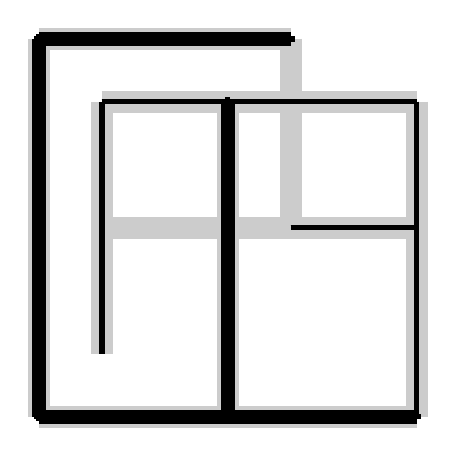
\begin{tikzpicture}[scale=0.8]%
\begin{scope}[shift={(0.5,{6.5})}, yscale=-1]%
\foreach \a/\b/\c/\d in {0/0/0/4,1/1/1/3,1/3/1/6,3/1/3/4,3/4/3/6,6/0/6/3,6/3/6/6,0/0/6/0,1/1/3/1,3/1/5/1,1/3/6/3,0/4/3/4,1/6/3/6,3/6/6/6} {%
\draw[line width=8pt, black!20!white] (\b,\a) -- (\d,\c);%
}%
\end{scope}%

\begin{scope}[shift={(0.5,{6.5})}, yscale=-1]%
\foreach \a/\b/\c/\d/\v in {0/0/0/4/2,1/1/1/3/1,1/3/1/6/1,3/4/3/6/1,6/0/6/3/2,6/3/6/6/2,0/0/6/0/2,1/1/3/1/1,3/1/5/1/1,1/3/6/3/2,1/6/3/6/1,3/6/6/6/1} {%
\foreach \k in {1, ..., \v}{%
\ifthenelse{\a = \c}{%
\draw[line width=2pt, yshift= {(\k - \v/2 - 0.5)*4pt}] (\b,\a) -- (\d,\c);%
}{%
\draw[line width=2pt, xshift= {(\k - \v/2 - 0.5)*4pt}] (\b,\a) -- (\d,\c);%
}%
} }%
\end{scope}%
\showCircleList{7}{7}{ {%
B, , , ,B, , ,%
 ,B, ,B, , ,B,%
 , , , , , , ,%
 ,B, , ,B, ,B,%
 , , , , , , ,%
 ,B, , , , , ,%
B, , ,B, , ,B%
} }{ 0.4 }%
\showList{7}{7}{ {%
4, , , ,2, , ,%
 ,2, ,4, , ,2,%
 , , , , , , ,%
 ,2, , ,1, ,3,%
 , , , , , , ,%
 ,1, , , , , ,%
4, , ,6, , ,3%
} }{ 0.8 }%
\end{tikzpicture}
\end{center}
\end{minipage}



\begin{itemize}
\item Les ponts sont de simples lignes droites, soit horizontales, soit verticales. Pas de passerelles coudées.
\item Les passerelles ne peuvent pas se croiser.
\item L'ensemble des îles forme un réseau connecté : il est toujours possible de passer d'une île à une autre en suivant les ponts.
\end{itemize}

Les bandes grises vous permettent de voir quelles îles sont potentiellement connectées. Il ne devrait pas y avoir de pont en dehors de ces bandes.
\end{tcolorbox}
}















\newcommand{\techtonicRules}{
\begin{tcolorbox}[colback=white]
\begin{center}
\begin{Large}
\textbf{Techtonic}
\end{Large}
\end{center}

Complétez la grille avec les chiffres manquants dans chaque zone entourée de gras, sachant que :\begin{itemize}
\item une zone de deux cases contient les chiffres 1 et 2, une zone de 3 cases contient les chiffres 1, 2, 3, etc.
\item Un chiffre placé dans une case ne peut se retrouver dans aucune des cases qui l'entourent (en diagonale y compris)
\end{itemize}
\end{tcolorbox}
}

\newcommand{\fillingRules}{
\begin{tcolorbox}[colback=white]
\begin{center}
\begin{Large}
\textbf{Filling}
\end{Large}
\end{center}

Remplissez entièrement la grille en plaçant dans chaque case vide un chiffre de 1 à 9 pour former des régions :\begin{itemize}
\item une région est formée de chiffres identiques et connexes. La taille d'une région doit correspondre au chiffre contenu dans les cases de cette région (a)
\item une région est composée de cases adjacentes (cases avec un côté commun, les diagonales ne sont pas acceptées) (b)
\item deux régions d'une même superficie ne peuvent être adjacentes (c)
\item toutes les régions de la solution ont au moins un de leur chiffre  apparent dans la grille initiale.
\end{itemize}
\begin{multicols}{3}
\begin{center}
(a) OUI

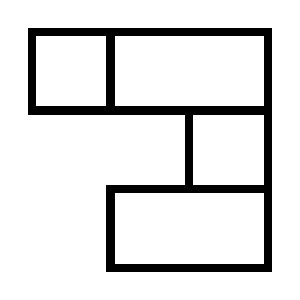
\begin{tikzpicture}[scale=1]
\plainGrid{3}
\showList{3}{3}{{
1,2,2,
3,3,1,
3,2,2
}}{1}
\draw[line width=3pt] (0,2) rectangle ++ (1,1) rectangle ++ (2,-1) rectangle ++ (-1,-1) ++ (-1,0) rectangle ++ (2,-1);
\end{tikzpicture}
\end{center}

\columnbreak
\begin{center}
(b) NON

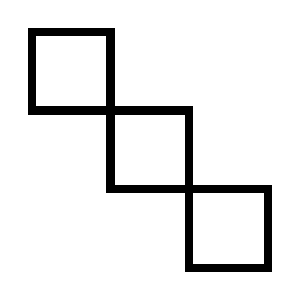
\begin{tikzpicture}[scale=1]
\plainGrid{3}
\showList{3}{3}{{
1,3,3,
3,2,3,
3,3,2
}}{1}
\draw[line width=3pt] (0,3) rectangle ++ (1,-1) rectangle ++ (1,-1) rectangle ++ (1,-1);
\end{tikzpicture}
\end{center}

\columnbreak
\begin{center}
(c) NON

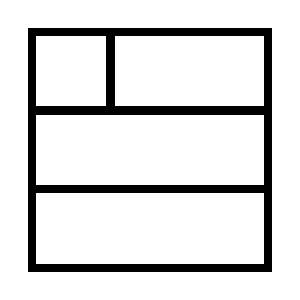
\begin{tikzpicture}[scale=1]
\plainGrid{3}
\showList{3}{3}{{
1,2,2,
3,3,3,
3,3,3
}}{1}
\draw[line width=3pt] (0,2) rectangle ++ (1,1) rectangle ++ (2,-1) rectangle ++ (-3,-1) rectangle ++ (3,-1);
\end{tikzpicture}
\end{center}
\end{multicols}
\end{tcolorbox}
}

\newcommand{\rikudoRules}{
\begin{tcolorbox}[colback=white]
\begin{minipage}{.5\linewidth}
\begin{center}
\begin{Large}
\textbf{Rikudo}
\end{Large}
\end{center}
\medskip

Compléter la grille avec des nombres qui se suivent, de 1 jusqu'au nombre final encadré, sachant que les nombres déjà placés servent de repères. Le signe $\blacklozenge$ relie deux cases qui contiennent des nombres consécutifs. Un seul chemin est possible et toutes les cases doivent être remplies.
\end{minipage}
\hfill
\begin{minipage}{.5\linewidth}
\begin{center}
\begin{tikzpicture}[scale=0.6]
\hexGrid{4}{
{30?02,29?3,25S,24,
31?15,28S,27,26,23,
1IS,32?04,33,17S,18,22S,
2,3S,34?1,B,16,19,21,
4,5S,35?4,15S,14,20S,
6,36IS,10S,11,13,
7,8,9S,12S
}
}{1}
\end{tikzpicture}
\end{center}
\end{minipage}
\end{tcolorbox}
}

\newcommand{\inequalRules}{
\begin{tcolorbox}[colback=white]
\begin{center}
\begin{Large}
\textbf{Inégal}
\end{Large}
\end{center}

% 4:0,0,0,0,0,0,0,0U,0,0R,0U,0U,0,0,0,3,

\begin{itemize}
\item Vous devez remplir une grille $N\times N$ avec les chiffres de $1$ à $N$. Chaque chiffre doit apparaître exactement une fois par ligne et par colonne.

\medskip
\emph{$N=4$ dans l'exemple. Remplir avec 1, 2, 3, 4.}

\item Les symboles indiquent une inégalité entre deux cases voisines.
\end{itemize}

\begin{minipage}{.5\linewidth}
\begin{center}
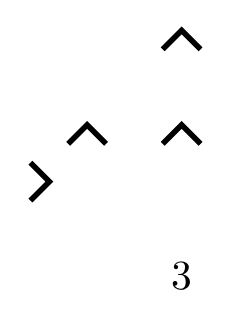
\begin{tikzpicture}[scale=1.2]%
\inequalGrid{4}%
\begin{scope}[shift={(0.5,3.5)}, yscale=-1]%
  \foreach \x/\y/\r in {3/1/270, 1/2/0, 2/2/270, 3/2/270} {%
    \begin{scope}[shift={(\x,\y)}, rotate=\r] \draw[line width=2pt] (.4,-.2) --++ (.2,.2) --++ (-.2,.2);\end{scope}%
  }%
\foreach \x/\y/\k in {3/3/3} { \draw (\x,\y) node[scale=1.5]{\k}; }%
\end{scope}%
\end{tikzpicture}
\end{center}

\end{minipage}
\hfill
\begin{minipage}{.5\linewidth}
\begin{center}
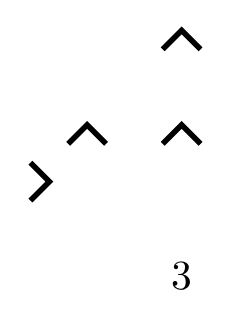
\begin{tikzpicture}[scale=1.2]%
\inequalGrid{4}%
\begin{scope}[shift={(0.5,3.5)}, yscale=-1]%
  \foreach \x/\y/\r in {3/1/270, 1/2/0, 2/2/270, 3/2/270} {%
    \begin{scope}[shift={(\x,\y)}, rotate=\r] \draw[line width=2pt] (.4,-.2) --++ (.2,.2) --++ (-.2,.2);\end{scope}%
  }%
\foreach \x/\y/\k in {3/3/3} {\draw (\x,\y) node[scale=1.5]{\k};}%
\end{scope}%
\showList{4}{4}{ {%
4,2,3,1,
3,4,1,2,
1,3,2,4,
2,1,4,3%
} }{1.5}%
\end{tikzpicture}
\end{center}

\end{minipage}
\end{tcolorbox}
}

\newcommand{\grecolatinRules}{
\begin{tcolorbox}[colback=white]
\begin{center}
\begin{Large}
\textbf{Carré Gréco-Latin}
\end{Large}
\end{center}

\begin{itemize}
\item Chaque case doit contenir deux éléments : une lettre (de A à E) et un chiffre (de 1 à 5).
\item Chaque lettre et chaque chiffre apparait une seule fois par ligne et par colonne.
\item Chaque combinaison lettre - chiffre (exemple A5)  est unique dans la grille.
\end{itemize}
\end{tcolorbox}
}

\newcommand{\fenceRules}{
\begin{tcolorbox}[colback=white]
\begin{minipage}{.65\linewidth}
\begin{center}
\begin{Large}
\textbf{Barrières}
\end{Large}
\end{center}

\begin{itemize}
\item Vous devez tracer une barrière qui fait \textbf{une} boucle en suivant les lignes du quadrillage.
\item La barrière ne se croise jamais.
\item Les cases numérotées indiquent le nombre de côtés de la case touchant la barrière.
\end{itemize}
\end{minipage}
\hfill
\begin{minipage}{.3\linewidth}
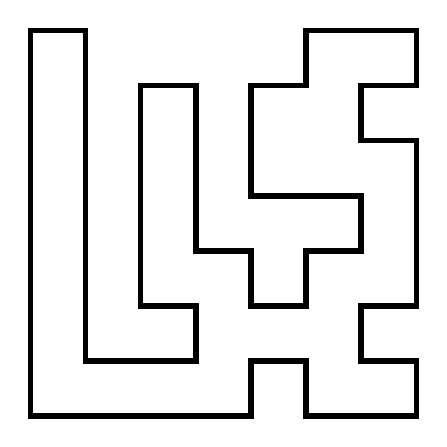
\begin{tikzpicture}[scale=.7]
\dottedGrid{7}
\showList{7}{7}{{
 , , ,0,2, ,3,
2, , ,2,2, ,3,
 , ,2, ,2, , ,
2,2,2,2, ,3, ,
 , ,2, ,3, , ,
2, , ,1, , ,3,
2,2,2,2, ,2, 
}}{1.4}
\draw[line width=2pt] (0,7) |- (4,0) |- (5,1) |- (7,0) |- (6,1) |- (7,2) |- (6,5) |- (7,6) |- (5,7) |- (4,6) |- (6,4) |- (5,3) |- (4,2) |- (3,3) |- (2,6) |- (3,2) |- (1,1) |- (0,7) -- cycle;
\end{tikzpicture}
\end{minipage}
\end{tcolorbox}
}

\newcommand{\kenkenRules}{
\begin{tcolorbox}[colback=white]
\begin{center}
\begin{Large}
\textbf{Kenken}
\end{Large}
\end{center}

\begin{itemize}
\item Vous devez remplir la grille $N\times N$ avec les chiffres de $1$ à $N$.
\item Tous les chiffres de $1$ à $N$ doivent apparaître une fois dans chaque ligne et chaque colonne.
\item Les chiffres de chaque région doivent permettre de réaliser le calcul indiqué.
\item Peu importe l'ordre dans une région. Par exemple pour $2\div$, on peut avoir :
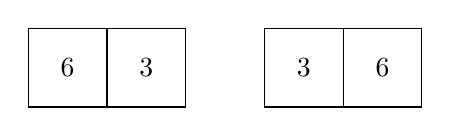
\begin{tikzpicture}
\draw (0,0) rectangle ++ (1,1) rectangle ++ (1,-1);
\draw (3,0) rectangle ++ (1,1) rectangle ++ (1,-1);
\draw (.5,.5) node{6} ++ (1,0) node{3} ++ (2,0) node{3} ++ (1,0) node{6};
\end{tikzpicture}
\end{itemize}
\end{tcolorbox}
}

\newcommand{\adjacentRules}{
\begin{tcolorbox}[colback=white]
\begin{minipage}{.59\linewidth}
\begin{itemize}
\item Toutes les lignes et colonnes ont $N$ cases blanches.
\item Vous devez compléter les cases blanches avec des chiffres de 1 à $N$.
\item Chaque ligne et chaque colonne doit contenir exactement une fois tous les chiffres de 1 à $N$.
\item Les symboles indiquent que les deux cases voisines sont des nombres consécutifs.
\item L'absence de symbole indique que les cases contiennent des nombres non consécutifs
\end{itemize}
\end{minipage}
\hfill
\begin{minipage}{.4\linewidth}

\begin{center}
\begin{Large}
\textbf{Adjacent}
\end{Large}
\end{center}

\begin{flushright}
\begin{tikzpicture}[scale=1]
\inequalGrid{5}

\adjacentH{5}{{
 0,1,1,0,
 1,0,0,0,
 1,0,1,0,
 1,1,1,1,
 0,0,0,0
}}
\adjacentV{5}{{
0,0,0,0,1,
1,1,1,0,1,
0,0,1,0,0,
0,1,0,0,1 
}}

\showList{5}{5}{{
2,5,4,3,1,
4,3,1,5,2,
5,4,2,1,3,
1,2,3,4,5,
3,1,5,2,4
}}{1.5}
\end{tikzpicture}
\end{flushright}
\end{minipage}
\end{tcolorbox}
}

\newcommand{\galaxiesRules}{
\begin{tcolorbox}[colback=white]

\begin{minipage}{.5\linewidth}
\begin{center}
\begin{Large}
\textbf{Galaxies}
\end{Large}
\end{center}

\begin{itemize}
\item Chaque cercle est une étoile qui est au centre de sa galaxie.
\item Une galaxie est une zone \textbf{connexe} et \textbf{symétrique} par rapport à son étoile.

Deux cases sont voisines si elles ont un bord en commun
\item Il ne doit pas rester de case libre à la fin et une case ne peut appartenir qu'a une galaxie.
\end{itemize}

\end{minipage}
\hfill
\begin{minipage}{.5\linewidth}
\begin{center}
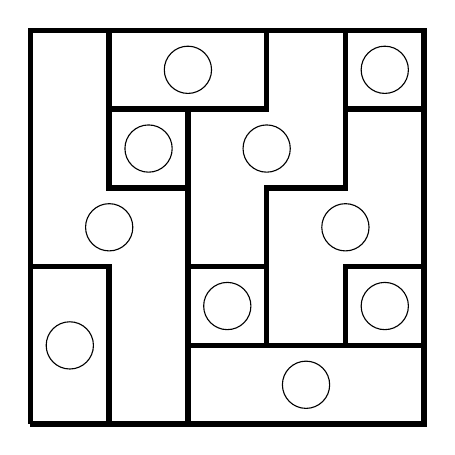
\begin{tikzpicture}[scale=1]
\dottedGrid{5}
\draw[line width=2pt] (1,4)--(3,4)--(3,5)--(1,5)--(1,4);
\draw[line width=2pt] (4,4)--(5,4)--(5,5)--(4,5)--(4,4);
\draw[line width=2pt] (1,3)--(2,3)--(2,4)--(1,4)--(1,3);
\draw[line width=2pt] (2,2)--(3,2)--(3,3)--(4,3)--(4,5)--(3,5)--(3,4)--(2,4)--(2,2);
\draw[line width=2pt] (1,0)--(2,0)--(2,3)--(1,3)--(1,5)--(0,5)--(0,2)--(1,2)--(1,0);
\draw[line width=2pt] (3,1)--(4,1)--(4,2)--(5,2)--(5,4)--(4,4)--(4,3)--(3,3)--(3,1);
\draw[line width=2pt] (2,1)--(3,1)--(3,2)--(2,2)--(2,1);
\draw[line width=2pt] (4,1)--(5,1)--(5,2)--(4,2)--(4,1);
\draw[line width=2pt] (0,0)--(1,0)--(1,2)--(0,2)--(0,0);
\draw[line width=2pt] (2,0)--(5,0)--(5,1)--(2,1)--(2,0);
\foreach \x/\y in {%
2.0/4.5,%
4.5/4.5,%
1.5/3.5,%
3.0/3.5,%
1.0/2.5,%
4.0/2.5,%
2.5/1.5,%
4.5/1.5,%
0.5/1.0,%
3.5/0.5%
} {\draw(\x,\y) circle(0.3);}
\end{tikzpicture}
\end{center}
\end{minipage}
\end{tcolorbox}
}

\newcommand{\thermometresRules}{
\begin{tcolorbox}[colback=white]

\begin{minipage}{.5\linewidth}
\begin{center}
\begin{Large}
\textbf{Thermomètres}
\end{Large}
\end{center}

\begin{itemize}
\item Il faut colorier les segments des thermomètres. Chaque case représente un segment. Ces segments coloriés représentent le mercure.
\item Le mercure doit partir du bulbe et monter continument jusqu'à un certain point. Un thermomètre peut être vide.
\item Les indices sur les bords indiquent le nombre de segments occupés par du mercure dans les lignes / colonnes correspondantes.
\end{itemize}

\end{minipage}
\hfill
\begin{minipage}{.5\linewidth}
\begin{center}
\def\bordsHBGD{ {4,3,3,3,3,1},{ },{4,1,2,1,5,4},{ } }
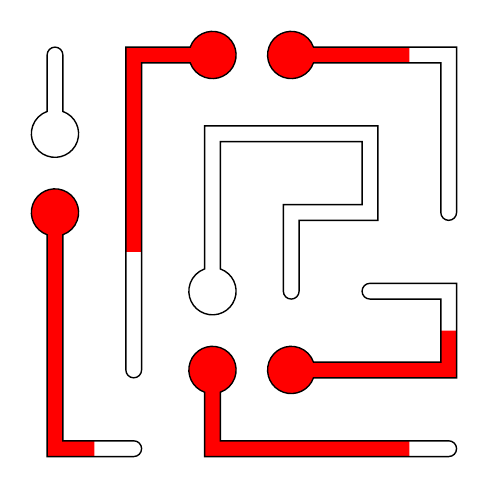
\begin{tikzpicture}[scale=1]
\plainGrid{6}
\sideItems{6}{6}{\bordsHBGD}{2}
\begin{scope}[shift={(0,6)}, yscale=-1]
\begin{scope}[shift={(.5,0.5)}]
\fill[red] (2,0) ++ (199.5:0.3) arc (199.5:520.5:0.3) -- (1.1,0.1) -- (1.1,1.0) -- (1.1,2.5) -- (0.9,2.5) -- (0.9,1.0) -- (0.9,-0.1) -- cycle;
\fill[red] (3,0) ++ (19.5:0.3) arc (19.5:340.5:0.3) -- (4.5,-0.1) -- (4.5,0.1) -- cycle;

\fill[red] (0,2) ++ (109.5:0.3) arc (109.5:430.5:0.3) -- (0.1,3.0) -- (0.1,4.0) -- (0.1,4.9) -- (0.5,4.9) -- (0.5,5.1) -- (-0.1,5.1) -- (-0.1,4.0) -- (-0.1,3.0) -- cycle;

\fill[red] (2,4) ++ (109.5:0.3) arc (109.5:430.5:0.3) -- (2.1,4.9) -- (3.0,4.9) -- (4.5,4.9) -- (4.5,5.1) -- (3.0,5.1) -- (1.9,5.1) -- cycle;
\fill[red] (3,4) ++ (19.5:0.3) arc (19.5:340.5:0.3) -- (4.0,3.9) -- (4.9,3.9) -- (4.9,3.5) -- (5.1,3.5) -- (5.1,4.1) -- (4.0,4.1) -- cycle;
\draw[line width=.5] (2,0) ++ (199.5:0.3) arc (199.5:520.5:0.3) -- (1.1,0.1) -- (1.1,1.0) -- (1.1,2.0) -- (1.1,3.0) -- (1.1,4.0) arc (0:180:0.1) -- (0.9,3.0) -- (0.9,2.0) -- (0.9,1.0) -- (0.9,-0.1) -- cycle;  
\draw[line width=.5] (3,0) ++ (19.5:0.3) arc (19.5:340.5:0.3) -- (4.0,-0.1) -- (5.1,-0.1) -- (5.1,1.0) -- (5.1,2.0) arc (0:180:0.1) -- (4.9,1.0) -- (4.9,0.1) -- (4.0,0.1) -- cycle;
\draw[line width=.5] (0,1) ++ (-70.5:0.3) arc (-70.5:250.5:0.3) -- (-0.1,0.0) arc (180:360:0.1) -- cycle;
\draw[line width=.5] (0,2) ++ (109.5:0.3) arc (109.5:430.5:0.3) -- (0.1,3.0) -- (0.1,4.0) -- (0.1,4.9) -- (1.0,4.9) arc (270:450:0.1) -- (-0.1,5.1) -- (-0.1,4.0) -- (-0.1,3.0) -- cycle;
\draw[line width=.5] (2,3) ++ (-70.5:0.3) arc (-70.5:250.5:0.3) -- (1.9,2.0) -- (1.9,0.9) -- (3.0,0.9) -- (4.1,0.9) -- (4.1,2.1) -- (3.1,2.1) -- (3.1,3.0) arc (0:180:0.1) -- (2.9,1.9) -- (3.9,1.9) -- (3.9,1.1) -- (3.0,1.1) -- (2.1,1.1) -- (2.1,2.0) -- cycle;
\draw[line width=.5] (2,4) ++ (109.5:0.3) arc (109.5:430.5:0.3) -- (2.1,4.9) -- (3.0,4.9) -- (4.0,4.9) -- (5.0,4.9) arc (270:450:0.1) -- (4.0,5.1) -- (3.0,5.1) -- (1.9,5.1) -- cycle;
\draw[line width=.5] (3,4) ++ (19.5:0.3) arc (19.5:340.5:0.3) -- (4.0,3.9) -- (4.9,3.9) -- (4.9,3.1) -- (4.0,3.1) arc (90:270:0.1) -- (5.1,2.9) -- (5.1,4.1) -- (4.0,4.1) -- cycle;
\end{scope}
\end{scope}
\end{tikzpicture}
\end{center}
\end{minipage}
\end{tcolorbox}
}


\newcommand{\nurikabeRules}{
\begin{tcolorbox}[colback=white]
\begin{center}
\begin{Large}
\textbf{Nurikabe}
\end{Large}
\end{center}

\begin{itemize}
\item Il faut noircir des cases. Les cases noircies représentent une rivière.
\item La rivière doit être entièrement connexe. Deux cases voisines sont connexes quand elles ont un bord en commun.
\item Les cases laissées en blancs représentent des îles. Une île est formée de cases blanche connexes dont exactement une avec un numéro. Ce numéro est le nombre de cases constituant l'ile. Deux îles ne doivent pas se toucher (aucun bord en commun)
\item Il ne doit pas y avoir de mare dans la rivière. La zone en noir ne doit pouvoir contenir aucun carré $2\times 2$.
\end{itemize}


\begin{minipage}{.5\linewidth}
\begin{center}
\begin{tikzpicture}[]
\nurikabe{5}{{
b,b,b,b,b,%
 , ,b, ,2,%
3,b,b,b,b,%
b,1,b, ,4,%
b,b,b, , %
}}{1}{0}
\end{tikzpicture}
\end{center}
\end{minipage}
\hfill
\begin{minipage}{.5\linewidth}
\begin{center}
\begin{tikzpicture}[]
\nurikabe{5}{{
b,b,b,b,b,%
 , ,b, ,2,%
3,b,b,b,b,%
b,1,b, ,4,%
b,b,b, , %
}}{1}{1}
\end{tikzpicture}
\end{center}
\end{minipage}


\end{tcolorbox}
}


\newcommand{\yingyangRules}{
\begin{tcolorbox}[colback=white]
\begin{center}
\begin{Large}
\textbf{Ying Yang}
\end{Large}
\end{center}

\begin{itemize}
\item Il faut remplir les cases avec un rond noir (N) ou blanc (B).
\item Deux cases se touchent si elles ont un bord en commun.
\item L'ensemble des cases B doivent être connexes. Même chose pour les cases N.
\item Il ne doit jamais y avoir de carré 2x2 tout blanc ou tout noir.
\end{itemize}



\begin{minipage}{.5\linewidth}
\begin{center}
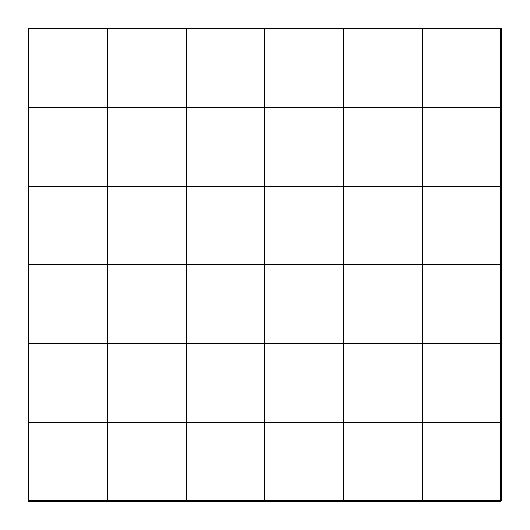
\begin{tikzpicture}[scale=1]%
\draw[line width=.5pt] (0,0) rectangle (6, 6);%
\draw[line width=.1pt] (0,0) grid[step=1] (6, 6);%
\showCircleList{6}{6}{ {%
 , , , , , ,%
 , , , , ,N,%
 , ,B, , , ,%
 ,B,N, ,B, ,%
 , , ,N, ,B,%
 , ,N, , , %
 } }{ 0.4 }%
\end{tikzpicture}
\end{center}
\end{minipage}
\hfill
\begin{minipage}{.5\linewidth}
\begin{center}
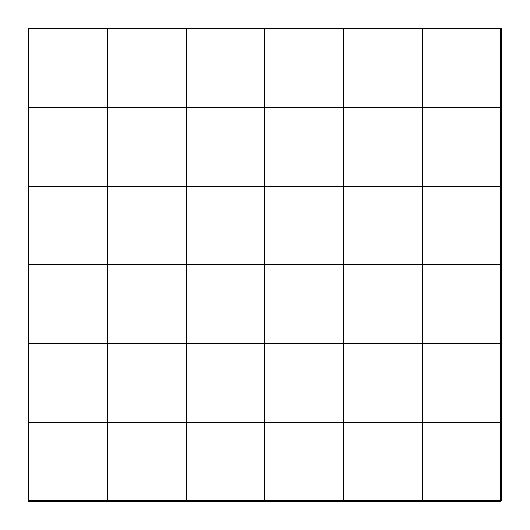
\begin{tikzpicture}[scale=1]%
\draw[line width=.5pt] (0,0) rectangle (6, 6);%
\draw[line width=.1pt] (0,0) grid[step=1] (6, 6);%
\connectListH{6}{6}{{%
1,3,3,3,3,2,%
0,0,0,1,2,0,%
0,1,3,2,1,2,%
0,0,0,1,3,2,%
0,0,1,3,2,0,%
1,3,2,1,3,2%
}}

\connectListV{6}{6}{{%
1,0,1,0,0,1,%
3,1,2,1,0,3,%
3,3,0,3,0,2,%
3,3,1,2,0,1,%
3,2,3,0,0,3,%
2,0,2,0,0,2%
}}

\showCircleList{6}{6}{ {%
N,N,N,N,N,N,%
N,B,N,B,B,N,%
N,B,B,B,N,N,%
N,B,N,B,B,B,%
N,B,N,N,N,B,%
N,N,N,B,B,B%
} }{ .3 }%

\showCircleList{6}{6}{ {%
 , , , , , ,%
 , , , , ,N,%
 , ,B, , , ,%
 ,B,N, ,B, ,%
 , , ,N, ,B,%
 , ,N, , , %
 } }{ 0.4 }%


\end{tikzpicture}
\end{center}

\end{minipage}

\medskip
\emph{Les traits reliant les disques ne sont pas nécessaires mais ils permettent de mieux voir les deux ensembles connexes.}
\end{tcolorbox}
}

\newcommand{\undeadRules}{
\begin{tcolorbox}[colback=white]
\begin{center}
\begin{Large}
\textbf{Undead}
\end{Large}
\end{center}

\begin{itemize}
\item Il faut placer différents types de morts-vivants. Des \textbf{G}hosts (fantômes), des \textbf{V}ampires et des \textbf{Z}ombies.

\item Chaque case doit être remplie par un mort-vivant et les valeurs données au dessus de la grille donnent l'effectif de chaque espèce
\item Les nombres sur les côtés indiquent le nombre d'individus que l'on verrait si on se plaçait là et que l'on regardait dans le miroir.

\medskip
\emph{L'œil donné en exemple indique un point de vue. De ce point là, on doit voir 4 morts-vivants sur la ligne tenant compte des reflets dans les miroirs.}

\item Un Zombie est toujours visible ; un vampire n'est pas visible quand on le voit à travers un ou plusieurs miroirs ; un fantôme n'est visible \textbf{que} si on le voit à travers un ou plusieurs miroirs.

\medskip
\emph{Dans l'exemple, en suivant la ligne de vue, on voit vampire et zombie avant le premier miroir, ce qui fait déjà 2. Après le miroir, on voit encore zombie, vampire, fantôme. Comme c'est dans un reflet (après miroir) le vampire n'est pas vu mais le fantôme et le zombie oui. On a donc bien un total de 4.}
\end{itemize}

\begin{minipage}{.5\linewidth}
\begin{center}
%id = tatham id = 4x4:3,3,4,bLbRbRLaRcL,1,2,1,3,0,4,0,0,1,5,0,2,2,2,2,3%
{\Large G = 3 \quad V = 3 \quad Z = 4 }%
\medskip%

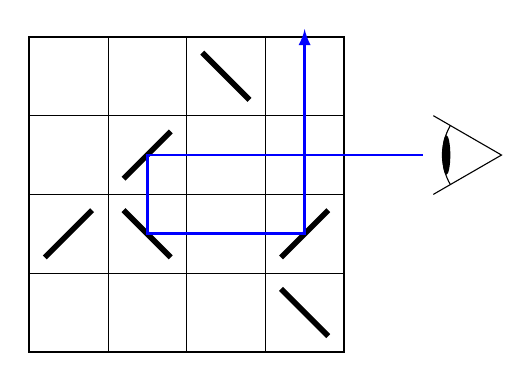
\begin{tikzpicture}[scale=1]%
\draw[line width=1pt] (0,0) rectangle (4, 4);%
\draw[line width=0.2pt] (0,0) grid[step=1] (4, 4);\begin{scope}[shift={(0,4)}, yscale=-1]%
\draw[line width=2pt] (2.5,0.5) ++(-.3,-.3) --++ (.6,.6);%
\draw[line width=2pt] (1.5,1.5) ++(.3,-.3) --++ (-.6,.6);%
\draw[line width=2pt] (0.5,2.5) ++(.3,-.3) --++ (-.6,.6);%
\draw[line width=2pt] (1.5,2.5) ++(-.3,-.3) --++ (.6,.6);%
\draw[line width=2pt] (3.5,2.5) ++(.3,-.3) --++ (-.6,.6);%
\draw[line width=2pt] (3.5,3.5) ++(-.3,-.3) --++ (.6,.6);%
\end{scope}%
\def\bordsHBGD{{1,2,1,3},{2,0,5,1},{3,2,2,2},{0,4,0,0}}%
\sideItems{4}{4}{\bordsHBGD}{2}%

\begin{scope}[shift={(6,2.5)},scale = 0.5, rotate=180]
\oeil
\end{scope}
\draw[blue, line width=1pt, ->, >=latex] (5,2.5) -- (1.5,2.5) -- (1.5,1.5) -- (3.5,1.5) -- (3.5,4.1);

\end{tikzpicture}
\end{center}
\end{minipage}
\hfill
\begin{minipage}{.5\linewidth}
\begin{center}
%id = tatham id = 4x4:3,3,4,bLbRbRLaRcL,1,2,1,3,0,4,0,0,1,5,0,2,2,2,2,3%
{\Large G = 3 \quad V = 3 \quad Z = 4 }%
\medskip%

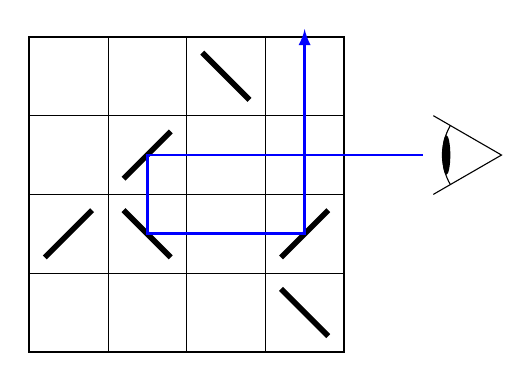
\begin{tikzpicture}[scale=1]%
\draw[line width=1pt] (0,0) rectangle (4, 4);%
\draw[line width=0.2pt] (0,0) grid[step=1] (4, 4);\begin{scope}[shift={(0,4)}, yscale=-1]%
\draw[line width=2pt] (2.5,0.5) ++(-.3,-.3) --++ (.6,.6);%
\draw[line width=2pt] (1.5,1.5) ++(.3,-.3) --++ (-.6,.6);%
\draw[line width=2pt] (0.5,2.5) ++(.3,-.3) --++ (-.6,.6);%
\draw[line width=2pt] (1.5,2.5) ++(-.3,-.3) --++ (.6,.6);%
\draw[line width=2pt] (3.5,2.5) ++(.3,-.3) --++ (-.6,.6);%
\draw[line width=2pt] (3.5,3.5) ++(-.3,-.3) --++ (.6,.6);%
\end{scope}%
\def\bordsHBGD{{1,2,1,3},{2,0,5,1},{3,2,2,2},{0,4,0,0}}%
\sideItems{4}{4}{\bordsHBGD}{2}%
\showList{4}{4}{{%
G,Z,,G,%
Z,,Z,V,%
,,Z,,%
V,G,V,%
}}{1}

\begin{scope}[shift={(6,2.5)},scale = 0.5, rotate=180]
\oeil
\end{scope}
\draw[blue, line width=1pt, ->, >=latex] (5,2.5) -- (1.5,2.5) -- (1.5,1.5) -- (3.5,1.5) -- (3.5,4.1);
\end{tikzpicture}
\end{center}
\end{minipage}

\textbf{Attention :} le vampire en ligne 2, colonne 4 est 2 fois dans la ligne de mire de sa ligne de miroirs. Il faut en tenir compte !

\end{tcolorbox}
}


\newcommand{\campingRules}{
\begin{tcolorbox}[colback=white]
\begin{center}
\begin{Large}
\textbf{Camping}
\end{Large}
\end{center}

Les cercles représentent des \textbf{arbres} dans un camping. Il faut placer des tentes en respectant ces règles :\begin{itemize}
\item Les indices sur les côtés indiquent le nombre de tentes par ligne / colonne.
\item Une tente est toujours voisine (bord commun) de l'arbre auquel elle est associée.
\item Une tente est toujours associée à exactement un arbre et réciproquement.
\item Deux tentes ne peuvent être voisines (par le bord et le coin)
\end{itemize}

\begin{minipage}{.5\linewidth}
\begin{center}
%id: tatham id = 5x5:ce_fae,1,1,1,0,2,2,1,0,1,1%
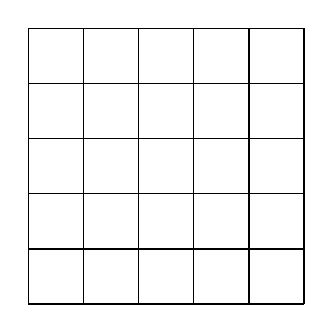
\begin{tikzpicture}[scale=.7]%
\draw[line width=0.5pt] (0,0) grid[step=1] (5,5);%
\showCircleList{5}{5}{ {%
 , , ,B, ,%
 , , , ,B,%
B, , , , ,%
 , ,B, ,B,%
 , , , , %
} }{ 0.2 }%
\def\bordsHBGD{{1,1,1,0,2},{ },{ },{2,1,0,1,1}}%
\sideItems{5}{5}{\bordsHBGD}{1}%
\end{tikzpicture}
\end{center}
\end{minipage}
\hfill
\begin{minipage}{.5\linewidth}
\begin{center}
%id: tatham id = 5x5:ce_fae,1,1,1,0,2,2,1,0,1,1%
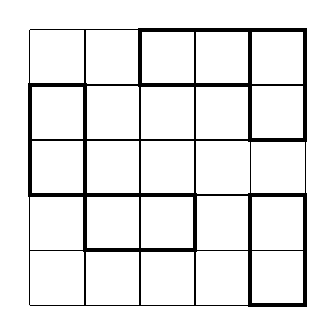
\begin{tikzpicture}[scale=.7]%
\draw[line width=0.5pt] (0,0) grid[step=1] (5,5);%
\showCircleList{5}{5}{ {%
 , , ,B, ,%
 , , , ,B,%
B, , , , ,%
 , ,B, ,B,%
 , , , , %
} }{ 0.2 }%
\def\bordsHBGD{{1,1,1,0,2},{ },{ },{2,1,0,1,1}}%
\sideItems{5}{5}{\bordsHBGD}{1}%
\showList{5}{5}{ {%
 , ,T, ,T,%
T, , , , ,%
 , , , , ,%
 ,T, , , ,%
 , , , ,T,%
} }{ 1 }%
\begin{scope}[shift={(0,5)}, yscale=-1]%
\foreach \y/\x in {0/2,3/1} {\draw[line width=1.5pt] (\x,\y ) rectangle ++ (2,1);}%
\foreach \y/\x in {0/4,1/0,3/4} {\draw[line width=1.5pt] (\x,\y) rectangle ++ (1,2);}%
\end{scope}%
\end{tikzpicture}
\end{center}
\end{minipage}

\textbf{Remarque :} en haut à droite, deux tentes voisinent un arbre. C'est autorisé ici puisque chacune de ses tentes est liée à un arbre différent. \quad Les rectangles ne sont pas requis mais ils permettent de voir clairement quel arbre est associé à quelle tente.

\end{tcolorbox}
}

\newcommand{\numbrixRules}{
\begin{tcolorbox}[colback=white]
\begin{center}
\begin{Large}
\textbf{Numbrix}
\end{Large}
\end{center}

Suit le principe du Rikudo mais avec des cases carrées. Il faut remplir les cases pour former un une suite de nombres. Voisinage par côté.

\begin{minipage}{.5\linewidth}
\begin{center}
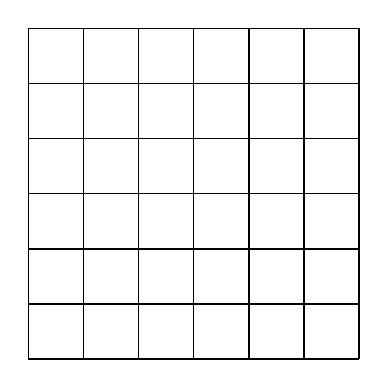
\begin{tikzpicture}[scale=.7]%
\draw[line width=0.5pt] (0,0) grid[step=1] (6,6);%
\showList{6}{6}{ {%
  ,31,  ,  ,06,  ,%
29,  ,  ,  ,  ,04,%
  ,  ,14,13,  ,  ,%
  ,  ,15,16,  ,  ,%
26,  ,  ,  ,  ,19,%
  ,24,  ,  ,21,  %
} }{ 1 }%
\end{tikzpicture}
\end{center}
\end{minipage}
\hfill
\begin{minipage}{.5\linewidth}
\begin{center}
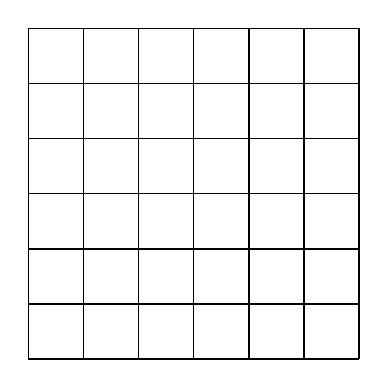
\begin{tikzpicture}[scale=.7]%
\draw[line width=0.5pt] (0,0) grid[step=1] (6,6);%
\showList{6}{6}{ {%
30,31,08,07,06,05,%
29,32,09,10,11,04,%
28,33,14,13,12,03,%
27,34,15,16,01,02,%
26,35,36,17,18,19,%
25,24,23,22,21,20%
} }{ 1 }%
\end{tikzpicture}
\end{center}
\end{minipage}
\end{tcolorbox}
}

\newcommand{\norinoriRules}{
\begin{tcolorbox}[colback=white]
\begin{center}
\begin{Large}
\textbf{Norinori}
\end{Large}
\end{center}

Un domino est un rectangle fait de deux cases grisées. Il faut placer les dominos dans la grille de sorte que :\begin{itemize}
\item chaque région ait exactement deux cases grisées,
\item deux dominos ne puissent se toucher que par les diagonales.
\end{itemize}
Vous devez griser des cases.

\medskip
\begin{minipage}{.5\linewidth}
\begin{center}
%id = 6x6:_dbba_a_a__a__bc_a__bc_a_3c__b%
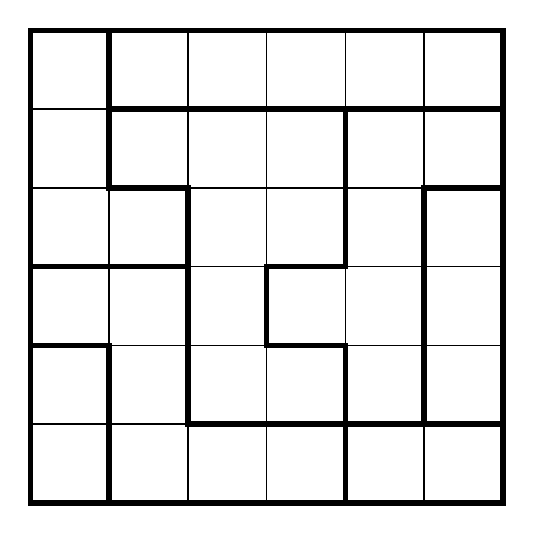
\begin{tikzpicture}[scale=1]%
\begin{scope}[shift={(0,6)}, yscale=-1]%
\draw[line width=.5pt] (0,0) grid[step=1] (6, 6);%

\draw[line width=2pt] (2,3) -- (0,3) -- (0,0) -- (1,0) -- (1,2) -- (2,2) -- cycle;%
\draw[line width=2pt] (6,1) -- (1,1) -- (1,0) -- (6,0) -- cycle;%
\draw[line width=2pt] (6,6) -- (4,6) -- (4,5) -- (6,5) -- cycle;%
\draw[line width=2pt] (4,5) -- (2,5) -- (2,2) -- (1,2) -- (1,1) -- (4,1) -- (4,3) -- (3,3) -- (3,4) -- (4,4) -- cycle;%
\draw[line width=2pt] (5,5) -- (5,2) -- (6,2) -- (6,5) -- cycle;%
\draw[line width=2pt] (4,6) -- (1,6) -- (1,4) -- (0,4) -- (0,3) -- (2,3) -- (2,5) -- (4,5) -- cycle;%
\draw[line width=2pt] (4,5) -- (4,4) -- (3,4) -- (3,3) -- (4,3) -- (4,1) -- (6,1) -- (6,2) -- (5,2) -- (5,5) -- cycle;%
\draw[line width=2pt] (0,6) -- (0,4) -- (1,4) -- (1,6) -- cycle;%
\end{scope}%
\end{tikzpicture}
\end{center}
\end{minipage}
\hfill
\begin{minipage}{.5\linewidth}
\begin{center}
%id = 6x6:_dbba_a_a__a__bc_a__bc_a_3c__b%
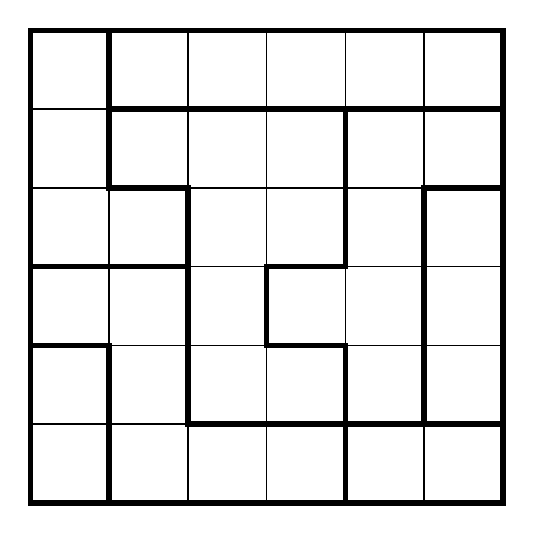
\begin{tikzpicture}[scale=1]%
\showColorList{6}{6}{ {%
k,k, , ,k, ,%
 , , , ,k, ,%
 ,k, ,k, ,k,%
 ,k, ,k, ,k,%
k, ,k, , , ,%
k, ,k, ,k,k%
} }%
\begin{scope}[shift={(0,6)}, yscale=-1]%

\draw[line width=.5pt] (0,0) grid[step=1] (6, 6);%

\draw[line width=2pt] (2,3) -- (0,3) -- (0,0) -- (1,0) -- (1,2) -- (2,2) -- cycle;%
\draw[line width=2pt] (6,1) -- (1,1) -- (1,0) -- (6,0) -- cycle;%
\draw[line width=2pt] (6,6) -- (4,6) -- (4,5) -- (6,5) -- cycle;%
\draw[line width=2pt] (4,5) -- (2,5) -- (2,2) -- (1,2) -- (1,1) -- (4,1) -- (4,3) -- (3,3) -- (3,4) -- (4,4) -- cycle;%
\draw[line width=2pt] (5,5) -- (5,2) -- (6,2) -- (6,5) -- cycle;%
\draw[line width=2pt] (4,6) -- (1,6) -- (1,4) -- (0,4) -- (0,3) -- (2,3) -- (2,5) -- (4,5) -- cycle;%
\draw[line width=2pt] (4,5) -- (4,4) -- (3,4) -- (3,3) -- (4,3) -- (4,1) -- (6,1) -- (6,2) -- (5,2) -- (5,5) -- cycle;%
\draw[line width=2pt] (0,6) -- (0,4) -- (1,4) -- (1,6) -- cycle;%
\end{scope}%
\end{tikzpicture}
\end{center}
\end{minipage}
\end{tcolorbox}
}